\chapter{من أنماط الزخم إلى الحقول الكمومية المحلية}

ما الحقل الكمومي، وكيف يرتبط بالجسيمات؟ الأداة الرياضية الأساسية هي المهتز التوافقي. يحتوي الحقل على أنماط اهتزاز ممكنة كثيرة، ويعني تكميم الحقل تجميع مهتز توافقي كمومي واحد لكل نمط. ويسهل رؤية هذا البناء أولًا في فضاء دوري منتهٍ، حيث تكوّن الأنماط المسموح بها قائمة منفصلة.

\section{الفضاء الدوري وأعداد الموجة المسموح بها}

خذ إحداثيًا مكانيًا واحدًا \(x\)، واعتبر النقاط المفصولة بمسافة \(L\) متطابقة. ويمكن تصور الفضاء على أنه دائرة محيطها \(L\). وهذه حيلة مفيدة لحجم منتهٍ. ففي مجال منتهٍ له طرفان، تنعكس الموجة السائرة عن الطرفين. أما في مجال دوري فيمكنها أن تتابع سيرها في أي من الاتجاهين من دون انعكاس. ويُحفَظ تناظر الإزاحة، ومن ثم انحفاظ الزخم، بينما تُزال مؤقتًا تعقيدات الحجم اللانهائي.

للموجة المستوية الشكل
\begin{equation}
e^{ikx}.
\end{equation}
وبعد دورة واحدة حول الدائرة لا بد أن تعود إلى قيمتها الأصلية. وبما أن الموجة تساوي \(1\) عند \(x=0\)، فإن الدورية تقتضي
\begin{equation}
e^{ikL}=1.
\end{equation}
لماذا يحقق مضاعف صحيح لـ \(2\pi\) هذا الشرط؟ تعطينا صيغة أويلر
\begin{align}
e^{i2\pi n}
&=\cos(2\pi n)+i\sin(2\pi n)\\
&=1,
\qquad n\in\mathbb Z.
\end{align}
يكون جيب التمام مساويًا لـ \(1\) ويكون الجيب مساويًا لـ \(0\) بعد أي عدد صحيح من الدورات. ولذلك،
\begin{equation}
kL=2\pi n,
\qquad
k=\frac{2\pi n}{L},
\qquad n\in\mathbb Z.
\end{equation}
والكمية \(k\) هي عدد الموجة. أما العدد الصحيح \(n\) فيُعيّن عدد موجة مسموحًا؛ وهو لا يعدّ الجسيمات بعد.

يمكن التعبير عن الشرط نفسه بدلالة الطول الموجي. فالطول الموجي هو المسافة التي يتقدم خلالها الطور دورة كاملة، لذا
\begin{equation}
k\lambda=2\pi,
\qquad
k=\frac{2\pi}{\lambda}.
\end{equation}
فالطول الموجي الكبير يقابله عدد موجة صغير، والطول الموجي القصير يقابله عدد موجة كبير. ويقول شرط الدورية إن عددًا صحيحًا من الأطوال الموجية يلائم الالتفاف حول الدائرة.

بالنسبة إلى موجة كمومية، يكون الزخم
\begin{equation}
p=\frac{h}{\lambda}
=\frac{2\pi\hbar}{\lambda}
=\hbar k.
\end{equation}
ومن ثم فإن \(k\) و\(p\) لا يختلفان إلا بالعامل \(\hbar\). وتصف القيم الموجبة والسالبة لـ \(k\) موجات تتحرك في اتجاهين متعاكسين وجسيمات ذات زخم في اتجاهين متعاكسين. وفي الوحدات التي فيها \(\hbar=1\)، من الشائع أن يُسمّى \(k\) زخمًا من دون مزيد من التفريق.

لكل \(k\) مسموح قد يوجد عدد ما من الكمّات في ذلك النمط. وهذا يُدخل عددًا صحيحًا ثانيًا:
\begin{equation}
n(k)=\text{number of quanta with wave number }k.
\end{equation}
ويُسمّى هذا عدد الإشغال. فالعدد الصحيح في \(k=2\pi n/L\) يوسم النمط، أما \(n(k)\) فيبيّن كم جسيمًا يشغل ذلك النمط. ويجب إعطاء أعداد الإشغال للقيم السالبة من \(k\) كما للقيم الموجبة منه.

\begin{classroomqa}
\lecturetimestamp{00:11:58}
\audiencequestion{هل \(k\) نفسه عدد صحيح؟}
\lecturerresponse{لا. عدد الموجة هو مضاعف صحيح لـ \(2\pi/L\): \(k=2\pi n/L\). والعدد الصحيح \(n\) في تلك الصيغة يوسم قيمة الزخم المسموح بها، وهو متميز عن عدد الإشغال \(n(k)\)، الذي يعدّ الكمّات في النمط.}
\end{classroomqa}

\section{حالات عدد الإشغال ومؤثرات الأنماط}

الحالة الكمومية متجه، أو عنصر خطي. ويمكن جمع متجهات الحالات وضربها في أعداد، وتؤثر فيها المؤثرات لتنتج متجهات حالة أخرى. وتمثَّل الكميات الحقيقية القابلة للرصد بمؤثرات هيرميتية. وهذه الحقائق الأولية مهمة هنا لأن حالة متعددة الجسيمات والحقل سيُبنيان من تراكيب خطية ومؤثرات.

لتكن
\begin{equation}
k_j=\frac{2\pi j}{L},
\qquad j\in\mathbb Z.
\end{equation}
وسم مناسب لحالة متعددة الجسيمات هو السلسلة الكاملة لأعداد الإشغال. وباستخدام الاختصار \(n_j\equiv n(k_j)\) للمدخلات المعروضة، نكتب
\begin{equation}
\big|\{n(k_j)\}\big\rangle
=
\big|\ldots,n_{-2},n_{-1},n_0,n_1,n_2,\ldots\big\rangle.
\end{equation}
ويمثل المدخل \(n(k_1)\) عدد الجسيمات في أول نمط ذي زخم موجب، ويمثل \(n(k_2)\) العدد في الثاني، وهكذا. وتمتد السلسلة بلا نهاية في الاتجاهين.

\begin{figure}[t]
\centering
\includegraphics[width=0.72\textwidth]{lecture_03_figure_02.png}
\caption{عدد الإشغال \(n(k)\) لنمط زخم مسموح.}
\lectureframe{00:15:04}
\end{figure}

كل نمط زخم هو مهتز توافقي. ولذلك فله مؤثر رفع ومؤثر خفض. والرمز المكتوب أولًا على صورة \(a^{+}(k)\) و\(a^{-}(k)\) سيُكتب على صورة \(a^\dagger(k)\) و\(a(k)\). وفعلهما هو
\begin{align}
a^\dagger(k)\big|\ldots,n(k),\ldots\big\rangle
&=
\sqrt{n(k)+1}\notag\\
&\quad{}\times
\big|\ldots,n(k)+1,\ldots\big\rangle,
\\
a(k)\big|\ldots,n(k),\ldots\big\rangle
&=
\sqrt{n(k)}\,
\big|\ldots,n(k)-1,\ldots\big\rangle.
\end{align}
يعمل المؤثر \(a^\dagger(k)\) على الخانة التابعة لـ \(k\)، فيرفع ذلك الإشغال بمقدار واحد، ويضرب الحالة في \(\sqrt{n(k)+1}\). ويخفض المؤثر \(a(k)\) الخانة نفسها ويعطي \(\sqrt{n(k)}\). ولكل زخم مسموح زوج كهذا.

\begin{figure}[t]
\centering
\includegraphics[width=0.58\textwidth]{lecture_03_figure_03.png}
\caption{مؤثرا الخلق والفناء المرتبطان بنمط الزخم \(k\).}
\lectureframe{00:17:14}
\end{figure}

\section{معاملات فورييه تصبح مؤثرات}

تبدأ الصلة بين مؤثرات المهتزات هذه وبين حقل بسلسلة فورييه كلاسيكية عادية. ويمكن كتابة حقل كلاسيكي عقدي على المجال الدوري على الصورة
\begin{align}
\psi(x)&=\sum_k \alpha(k)e^{ikx},\\
\psi^*(x)&=\sum_k \alpha^*(k)e^{-ikx},
\end{align}
حيث يكون كل مجموع على القيم المسموح بها \(k=2\pi n/L\). وهذا يكافئ توسيع الحقل في جيوب وجيوب تمام.

للحقل العقدي جزء حقيقي وجزء تخيلي. ويعكس مرافقه العقدي إشارة الجزء التخيلي، وتصبح \(e^{ikx}\) هي \(e^{-ikx}\). إن تحديد جميع المعاملات \(\alpha(k)\) يحدد الحقل الكلاسيكي. ولا حاجة إلى تحديد \(\alpha^*(k)\) استقلالًا ما دامت \(\alpha(k)\) معلومة، لكن الجزأين الحقيقي والتخيلي لكل معامل هما كميتان حقيقيتان منفصلتان. ويمكن قياسهما بوصفهما سعتي مركبتي فورييه المناظرتين. وبهذا المعنى يجمع المعامل العقدي مقدارين كلاسيكيين قابلين للرصد.

يستبدل التكميم معاملات فورييه الكلاسيكية هذه بمؤثرات. إن علامة المساواة العادية ستجعل أشياء من نوعين مختلفين متطابقة، لذا من الأفضل كتابة قاعدة إحلال:
\begin{equation}
\alpha(k)\rightsquigarrow a(k),
\qquad
\alpha^*(k)\rightsquigarrow a^\dagger(k).
\end{equation}
ومع اختيار متسق لإشارات فورييه، تُعرَّف الحقول الكمومية كما يلي
\begin{align}
\Psi(x)&=\sum_k a(k)e^{ikx},\\
\Psi^\dagger(x)&=\sum_k a^\dagger(k)e^{-ikx}.
\end{align}
\editorialnote{يغيّر النقاش الشفهي اصطلاح إشارات فورييه ثم يشكك فيه لاحقًا. والزوج المترافق المستخدم هنا هو الاصطلاح الظاهر في توسيع الحقل الأوضح وفي حساب حالة الموضع: تحمل \(\Psi\) العامل \(e^{ikx}\) وتحمل \(\Psi^\dagger\) العامل \(e^{-ikx}\). إن عكس جميع الإشارات على نحو متسق يصف البناء نفسه.}

في الوقت الراهن، هذا تعريف: الحقل الكمومي هو مجموع فورييه معاملاته مؤثرات. وكان تبرير أكمل سيتعيّن عليه أن يبيّن كيف تعيد هذه المؤثرات إنتاج المعاملات الكلاسيكية في حد مناسب، وهذا يتطلب بعض الديناميكيات. ويؤجَّل هذا السؤال. أما ما هو واضح بالفعل فهو أن الحقل نفسه مؤثر، وأن العلاقات بين معاملات فورييه الخاصة به هي علاقات الخلق والفناء للمهتزات التوافقية.

\begin{classroomqa}
\lecturetimestamp{00:26:48}
\audiencequestion{هل يعني إدخال مؤثري الخلق والفناء أن الديناميكيات تخلق الجسيمات وتفنيها بالضرورة؟}
\lecturerresponse{لا. فهذه المؤثرات عمليات رياضية تغيّر أعداد الإشغال. أما ما إذا كانت قوانين الطبيعة تغيّر عدد الجسيمات فعليًا، فذلك سؤال يتعلق بالديناميكيات. وإذا سمحت الديناميكيات بمثل هذه التغييرات، فإن هذه المؤثرات توفر اللغة الطبيعية لوصفها.}
\end{classroomqa}

\section{التشتت وعدد الجسيمات المتغيّر}

لننظر أولًا في عملية لا تغيّر عدد الجسيمات. افترض أن الجسيم الوحيد الموجود ابتدائيًا له الزخم \(k_7\). وفي ترميز عدد الإشغال، تكون حالته ذات \(1\) في الخانة السابعة وأصفار في كل موضع آخر:
\begin{equation}
|k_7\rangle
=
|\ldots,0,\underset{k_7}{1},0,\ldots\rangle.
\end{equation}
وتغيّر عملية تشتت زخمه من \(k_7\) إلى \(k_9\). والمؤثر الذي يُحدث هذا التغير على وجه الدقة هو
\begin{equation}
a^\dagger(k_9)a(k_7).
\end{equation}
يعمل المؤثر الواقع إلى اليمين أولًا: فهو يزيل الجسيم من الخانة \(k_7\). ثم يخلق المؤثر الواقع إلى اليسار جسيمًا في الخانة \(k_9\).

\begin{classroomqa}
\lecturetimestamp{00:31:37}
\audiencequestion{أين تدخل عوامل الجذر التربيعي في هذه العملية \(k_7\to k_9\)؟}
\lecturerresponse{عامل الفناء هو \(\sqrt{n(k_7)}=\sqrt{1}=1\). وبعد هذه الإزالة تصبح المنظومة في الحالة التي كل خاناتها أصفار. وبما أن النمط \(k_9\) فارغ، فإن عامل الخلق هو \(\sqrt{n(k_9)+1}=\sqrt{1}=1\). ومن ثم لا يغيّر أي من العاملين المعامل العددي في مثال الجسيم الواحد هذا.}
\end{classroomqa}

لننفذ الخطوتين كلتيهما. يعطي الفناء
\begin{align}
a(k_7)|k_7\rangle
&=
\sqrt{1}\,|\ldots,0,0,0,\ldots\rangle\\
&=|0\rangle.
\end{align}
والحالة التي كل خاناتها أصفار هي الخلاء. وهي الحالة الخالية من الجسيمات، وهي أيضًا في هذه المجموعة البسيطة من المهتزات الحالة القاعية. ثم يعطي الخلق في النمط الفارغ \(k_9\)
\begin{equation}
a^\dagger(k_9)|0\rangle
=\sqrt{0+1}\,|k_9\rangle
=|k_9\rangle.
\end{equation}
ولذلك،
\begin{equation}
a^\dagger(k_9)a(k_7)|k_7\rangle=|k_9\rangle.
\end{equation}
وعلى مستوى الخانات، لم يفعل \(1\) الوحيد سوى الانتقال من نمط الزخم السابع إلى التاسع. ولأن أي إشغال لم يتجاوز الواحد قط، كان كل من عاملي الجذر التربيعي مساويًا للواحد. وسيصبحان مهمين حالما يدخل في الأمر نمط مشغول من قبل.

يمكن أيضًا وصف هذه العملية من واحد إلى واحد في ميكانيكا الكم العادية لجسيم واحد: إذ يغيّر جسيم واحد زخمه. وتصبح لغة أعداد الإشغال لا غنى عنها عندما يمكن أن يتغير عدد الجسيمات. فمثلًا،
\begin{equation}
a^\dagger(k_9)a^\dagger(k_{16})a(k_7)|k_7\rangle
=|k_9,k_{16}\rangle
\end{equation}
يصف التحول الرياضي من جسيم داخل واحد في النمط \(k_7\) إلى جسيمين خارجين، أحدهما في \(k_9\) والآخر في \(k_{16}\). وقد يمتص هدفٌ الجسيمَ الداخل، ويبعث الجسيمين الخارجين، ويتحمل ما يلزم من ارتداد. ولا يمكن تمثيل مثل هذه العملية في فضاء هلبرت مقيَّد بجسيم واحد، لكنها تنسجم طبيعيًا مع فضاء حالات يمكن أن تتغير فيه أعداد الإشغال. وليس التعبير المؤثري في حد ذاته قانونًا للطبيعة؛ بل هو اللغة التي يمكن أن يُكتب بها قانون يغيّر عدد الجسيمات.

\section{مؤثِّر حقلي عند نقطة}

ماذا يخلق مؤثِّر فضاء الموضع \(\Psi^\dagger(x)\)؟ تشكّل الحالات الكمومية فضاءً خطيًا: إذ يمكن جمع حالات الزخم بمعاملات مركبة لتكوين حالة جديدة. ابدأ من الخلاء. وبما أن كل نمط فارغ،
\begin{equation}
\Psi(x)|0\rangle=0.
\end{equation}
فإن الصفر في الطرف الأيمن هو المتجه الصفري: إذ لا يستطيع مؤثِّر الإفناء أن يجد أي جسيم ليفنيه.

يعمل الحقل المرافق على نحو مختلف:
\begin{align}
\Psi^\dagger(x)|0\rangle
&=\sum_k e^{-ikx}a^\dagger(k)|0\rangle\\
&=\sum_k e^{-ikx}|k\rangle,
\end{align}
حيث إن
\begin{equation}
|k\rangle=a^\dagger(k)|0\rangle
\end{equation}
هي حالة الجسيم الواحد ذات الزخم \(\hbar k\).

\begin{figure}[t]
\centering
\includegraphics[width=0.70\textwidth]{lecture_03_figure_05.png}
\caption{الحالة الشكلية في فضاء الموضع \(\Psi^\dagger(x)|0\rangle\) موسَّعة في حالات الزخم أحادية الجسيم.}
\lectureframe{00:43:16}
\end{figure}

من الناحية الشكلية، وبإهمال عامل التطبيع، يكون المجموع هو حالة الموضع المعممة في ميكانيكا الكم لجسيم واحد.\footnote{مع وجود عدد لا نهائي من أنماط الزخم، تكون حالة الموضع المتموضعة تمامًا غير قابلة للتطبيع. وبدلًا من ذلك، فإن فرض قطع منتهٍ للزخم ثم تطبيع المجموع المبتور يعطي حزمة موجية متموضعة بحدة ومتمركزة عند \(x\).} وتنتج الحالات الذاتية للزخم، مقترنةً بالمعاملات \(e^{-ikx}\)، تموضعًا عند \(x\). وبهذا المعنى الشكلي،
\begin{equation}
\Psi^\dagger(x)\ \text{creates a particle at position }x,
\end{equation}
بينما
\begin{equation}
\Psi(x)\ \text{annihilates a particle at position }x.
\end{equation}
يخلق مؤثِّر النمط \(a^\dagger(k)\) جسيمًا ذا زخم محدد. أما المؤثِّر الحقلي \(\Psi^\dagger(x)\) فيخلق التراكب المتماسك لحالات الزخم المسموح بها، المتموضع شكليًا عند \(x\).

في المجموع الشكلي غير المطبَّع، يكون مقدار كل معامل \(e^{-ikx}\) مساويًا للواحد. ومع وجود قطع منتهٍ، تكون للحالة المبتورة المطبَّعة معاملات متساوية المقدار للزخوم المحتفَظ بها، بينما تنتج أطوارها حزمةً موجية متموضعة بحدة قرب \(x\). وهذه هي الصلة الأولية بين الحقل الكمومي والجسيمات.

ومع تجاهل تعقيدات النسبية الخاصة في الوقت الحاضر، فإن \(\Psi^\dagger(x)\) يخلق جسيمًا عند \(x\) في هذا النموذج. وتتطلب الحقول النسبية مزيدًا من التنقيح، لكن توسع فورييه ذي القيم المؤثرية والتمييز بين مؤثرات أنماط الزخم ومؤثرات فضاء الموضع يظلان أساسيين.

\begin{classroomqa}
\lecturetimestamp{00:44:59}
\audiencequestion{هل \(x\) نقطة على الدائرة الدورية، وماذا يحدث عندما تكبر الدائرة؟}
\lecturerresponse{نعم. في النموذج المنتهي، يكون \(x\) نقطة على الدائرة. وتفصل بين الأعداد الموجية المسموح بها المتجاورة مسافة \(2\pi/L\). ومع ازدياد \(L\) تصغر تلك المسافة، ولذلك توجد لكل زخم مطلوب قيمة مسموح بها قريبة منه على نحو اعتباطي. وفي حد الحجم اللانهائي، تُستبدل المجاميع على \(k\) بتكاملات على \(k\). ومن المفيد فهم المجاميع المتقطعة أولًا.}
\end{classroomqa}

\section{تفاعلات جسيمية محلية}

بمجرد أن يُفسَّر \(\Psi(x)\) و\(\Psi^\dagger(x)\) على أنهما يفنيان ويخلقان جسيمات عند نقطة، يمكن التعبير عن المحلية مباشرةً. تخيل أن جسيمًا يمتصه هدف متموضع بحدة عند \(x\)، بينما يظهر فجأةً جسيم خارج قرب Alpha Centauri وآخر قرب Betelgeuse. مثل هذا التفاعل غير محلي: فأحداثه المتباعدة لا يمكن وصلها بانتشار عادي.

يمكن أولًا إضعاف الشرط والسماح بانبعاث الجسيمات الخارجة في مكان ما داخل منطقة صغيرة حول الهدف. لكن المثالية المحلية الدقيقة أقوى من ذلك: فإذا امتص الجسيم الداخل عند \(x\)، خُلقت الجسيمات الخارجة عند تلك النقطة نفسها. أما استخدام حقول مقوَّمة عند نقاط متباعدة فسيصف بدلًا من ذلك جداء مؤثرات غير محلي. ولذلك تكون العملية المحلية من واحد إلى اثنين هي
\begin{equation}
\Psi^\dagger(x)\Psi^\dagger(x)\Psi(x).
\end{equation}
يُفني الحقل الواقع أقصى اليمين الجسيمَ الداخل عند \(x\)؛ ويخلق الحقلان الواقعان إلى يساره جسيمين خارجين هناك.\footnote{يتبع المخطط المحلي من واحد إلى اثنين التفاعل الموصوف عند 00:47:38--00:49:13.}

\begin{figure}[t]
\centering
\begin{tikzpicture}[scale=1.0]
\draw[->] (-2.2,0) -- (0,0);
\fill (0,0) circle (2.2pt);
\draw[->] (0,0) -- (2.0,1.1);
\draw[->] (0,0) -- (2.0,-1.1);
\node at (-1.25,0.3) {$k_{\mathrm{initial}}$};
\node[right] at (0.05,0.05) {$x$};
\node at (1.48,1.34) {$\ell$};
\node at (1.48,-1.34) {$m$};
\end{tikzpicture}
\caption{يُمتص جسيم داخل واحد عند \(x\)، ويُخلق جسيمان خارجان عند النقطة نفسها.}
\end{figure}

لتكن الحالة الداخلة محتويةً على جسيم واحد ذي عدد موجي محدد \(k_{\mathrm{initial}}\). ولتحديد الزخوم الخارجة، عوِّض بتوسعات الحقول المحلية في فضاء الزخم. ومن المهم فصل وسم زخم ثابت عن مؤشر جمع صوري. اكتب
\begin{align}
\Psi(x)&=\sum_q a(q)e^{iqx},\\
\Psi^\dagger(x)&=\sum_\ell a^\dagger(\ell)e^{-i\ell x}.
\end{align}
المؤشر \(q\) مجموع عليه، في حين أن \(k_{\mathrm{initial}}\) يوسم النمط الداخل المشغول المعين. كما تتطلب النسختان من \(\Psi^\dagger(x)\) أيضًا مؤشرين صوريين مستقلين، لنقل \(\ell\) و\(m\). وإعادة استخدام مؤشر واحد ستربط على نحو غير صحيح بين مجموعين مستقلين. وهنا \(\ell\) و\(m\) عددان موجيان؛ ولا يرمز \(m\) إلى الكتلة.

ومن التصورات الملموسة أن فوتونًا يصطدم بذرة متموضعة عند \(x\)، ثم يغادر فوتونان تلك النقطة. غير أن الحقل البسيط المستخدم هنا أنسب لجسيمات غير نسبية منه لحقل فوتوني نسبي تمامًا، لذلك فإن لغة الفوتونات هنا لا تؤدي إلا دور توضيح تتبّع المؤثرات.

يعمل حقل الإفناء أولًا:
\begin{align}
\Psi(x)|k_{\mathrm{initial}}\rangle
&=\sum_q e^{iqx}a(q)a^\dagger(k_{\mathrm{initial}})|0\rangle.
\end{align}
ينعدم كل حد إلا الحد الذي فيه \(q=k_{\mathrm{initial}}\). فلا بد لمؤثِّر الإفناء أن يجد جسيمًا في نمطه نفسه. ومن ثم
\begin{equation}
\Psi(x)|k_{\mathrm{initial}}\rangle
=e^{ik_{\mathrm{initial}}x}|0\rangle.
\end{equation}
ثم يعطي حقلا الخلق
\begin{align}
&\Psi^\dagger(x)\Psi^\dagger(x)\Psi(x)
|k_{\mathrm{initial}}\rangle
\\
&\quad=
e^{ik_{\mathrm{initial}}x}
\sum_{\ell,m}
e^{-i\ell x}e^{-imx}
a^\dagger(\ell)a^\dagger(m)|0\rangle
\\
&\quad=
\sum_{\ell,m}
e^{i(k_{\mathrm{initial}}-\ell-m)x}
a^\dagger(\ell)a^\dagger(m)|0\rangle.
\end{align}
وإذا كان \(\ell\) و\(m\) غير متساويين، أمكن الدلالة على الحالة بـ \(|\ell,m\rangle\): إذ يشغل جسيم واحد كلًّا من النمطين. والنتيجة النهائية هي مجموع على جميع تشكيلات الزخم لجسيمين من هذا النوع، مع طور تحدده الزخوم الداخلة والخارجة.

\begin{classroomqa}
\lecturetimestamp{01:00:36}
\audiencequestion{هل يتبادل مؤثرا الخلق هذان؟}
\lecturerresponse{نعم. جميع مؤثرات الخلق تتبادل فيما بينها، وجميع مؤثرات الإفناء تتبادل فيما بينها. ويتبادل مؤثِّر خلق ومؤثِّر إفناء عندما يشيران إلى نمطين مختلفين؛ أما في النمط نفسه فمبادلهما غير صفري.}
\end{classroomqa}

\begin{classroomqa}
\lecturetimestamp{01:01:34}
\audiencequestion{هل ينبغي أن يحقق الزخمان الخارجان حفظ الزخم؟}
\lecturerresponse{ليس من الضروري أن يحقق الجسيمان المعروضان حفظ الزخم بمفردهما، لأن الذرة أو الهدف يمكن أن يرتدّ. والفرق \(k_{\mathrm{initial}}-\ell-m\) هو الزخم المنقول إلى الهدف. والزخم الكلي، بما في ذلك الهدف، هو الكمية المحفوظة.}
\end{classroomqa}

بما أن المعامل \(e^{i(k_{\mathrm{initial}}-\ell-m)x}\) طور صرف، فإن مقداره يساوي واحدًا. وقد يوحي هذا للوهلة الأولى بأوزان احتمالية متساوية لجميع الأزواج \((\ell,m)\). ولكن ثمة تحفّظًا مهمًا عندما يتطابق الوسمان.

إذا كان \(\ell=m\)، فإن مؤثِّر الخلق الأول يضع جسيمًا واحدًا في النمط \(m\)، ثم يعمل الثاني على نمط سبق أن شُغل مرة واحدة:
\begin{align}
a^\dagger(m)a^\dagger(m)|0\rangle
&=a^\dagger(m)|1_m\rangle\\
&=\sqrt{2}\,|2_m\rangle.
\end{align}
ومن ثم فإن الخلق المزدوج في نمط واحد له سعة إضافية \(\sqrt{2}\). ويولّد تربيع السعة عاملًا مقداره \(2\) في الاحتمال.

\begin{classroomqa}
\lecturetimestamp{01:04:54}
\audiencequestion{هل يجب أن يختلف \(\ell\) و\(m\) بمقدار واحد لأن معامل الخلق يحتوي على \(n+1\)؟}
\lecturerresponse{لا. فالرمزان \(\ell\) و\(m\) يوسمان أنماط الزخم. أما \(n\) في \(\sqrt{n+1}\) فهو عدد إشغال النمط المعين الذي يعمل عليه مؤثِّر الخلق. ووسوم الزخم وأعداد الجسيمات أعداد صحيحة متميزة.}
\end{classroomqa}

\begin{figure}[t]
\centering
\includegraphics[width=0.92\textwidth]{lecture_03_figure_06.png}
\caption{توسيع فضاء الزخم للسعة المحلية لتحويل جسيم واحد إلى جسيمين.}
\lectureframe{01:05:44}
\end{figure}

الجسيمات في هذا البناء متطابقة. ولذلك فإن \(\sqrt{2}\) عامل إشغال بوزوني، لا وسم يميز جسيمًا أول عن ثانٍ. ويبدو أن تربيعه يجعل، مبدئيًا، ناتج الزخمين المتساويين أكثر احتمالًا بمرتين من حد واحد ذي زخمين غير متساويين. غير أن هذه المقارنة ستحتاج إلى إعادة نظر بعد عدّ حدود المجموع المزدوج بعناية.

\begin{classroomqa}
\lecturetimestamp{01:06:43}
\audiencequestion{في تفاعل معقد، كيف يُختار ترتيب مؤثرات الخلق والإفناء؟}
\lecturerresponse{يُسمّى التعبير الذي تكون فيه جميع مؤثرات الخلق إلى اليسار وجميع مؤثرات الإفناء إلى اليمين مرتبًا ترتيبًا عاديًا. وفي تلك الصورة، تزيل المؤثرات الواقعة أقصى اليمين أولًا الجسيمات الداخلة، ثم تخلق المؤثرات الباقية الجسيمات الخارجة.}
\end{classroomqa}

إن إعادة ترتيب زوج مختلط من مؤثري الإنشاء--الإفناء ليست عموماً مجرد تبديل بسيط: بل يجب أن يُستخدَم المبدِّل، وللنمط نفسه ينتج عن ذلك حد إضافي.\footnote{هذا التقييد المتعلق بالمبدِّل هو تصويب تحريري للمناقشة غير الرسمية للترتيب العادي عند 01:06:43.}

\begin{classroomqa}
\lecturetimestamp{01:07:30}
\audiencequestion{إذا كانت جميع سعات الزخم لها المقدار نفسه، فماذا تعني عبارة مثل ``أكثر احتمالاً بمرتين''؟}
\lecturerresponse{ضع في ذهنك التجويف المحدود. فالزخوم المسموح بها فيه متقطعة، ولذلك يمكن مقارنة الاحتمالات نمطاً بنمط. والمقارنة ليست بين احتمالات نقاط معزولة في متصل.}
\end{classroomqa}

عند \(\ell\ne m\)، يحتوي المجموع المزدوج غير المقيَّد على كلا الحدين المرتَّبين
\begin{equation}
a^\dagger(\ell)a^\dagger(m)|0\rangle
\quad\text{and}\quad
a^\dagger(m)a^\dagger(\ell)|0\rangle.
\end{equation}

\begin{classroomqa}
\lecturetimestamp{01:08:24}
\audiencequestion{عندما \(\ell\ne m\)، هل تظهر الحالة النهائية نفسها مرتين في المجموع المزدوج، مرة على صورة \((\ell,m)\) ومرة على صورة \((m,\ell)\)؟}
\lecturerresponse{نعم. إذا كان \(\ell\ne m\)، فإن الحدين \((\ell,m)\) و\((m,\ell)\) يردان كلاهما، وبما أن مؤثرات الإنشاء تتبادل فإنهما يصفان الحالة الفيزيائية نفسها.}
\end{classroomqa}

الحدان المرتبان متساويان، لذا يجب التعامل مع تطبيع الحالة وهذا العدّ المزدوج قبل إجراء مقارنة كمية بين القنوات. والاستنتاج الجبري الموثوق أضيق من ذلك، لكنه كافٍ لما يلي: فالإنشاء في نمط مشغول سلفاً بـ\(n\) من البوزونات المتماثلة يولِّد العامل \(\sqrt{n+1}\).

\section{الانبعاث التلقائي والمحثوث}

مثال أنقى يعزل عامل الجذر التربيعي. افترض أن جسماً متموضعاً عند \(x\) يصدر فوتوناً واحداً. إذا بدأ حقل الفوتون في حالة الفراغ، فإن الحالة الخارجة هي
\begin{align}
\Psi^\dagger(x)|0\rangle
&=\sum_k e^{-ikx}a^\dagger(k)|0\rangle\\
&=\sum_k e^{-ikx}|k\rangle.
\end{align}
ضمن هذا النموذج المبسَّط، تكون جميع الزخوم ذات المقدار نفسه للسعة. ومع عدم وجود فوتونات مسبقاً، يكون الانبعاث تلقائياً.

الآن افترض أن هناك بالفعل فوتوناً واحداً في النمط \(\ell\). إن تأثير حقل الإنشاء الموضعي نفسه يعطي نوعين من الحدود:
\begin{equation}
\Psi^\dagger(x)|\ell\rangle
=
\sum_{k\ne\ell}e^{-ikx}|k,\ell\rangle
+e^{-i\ell x}\sqrt{2}\,|2_\ell\rangle.
\end{equation}
عند \(k\ne\ell\)، ينشئ المؤثر في نمط فارغ، لذا يكون المعامل \(\sqrt{0+1}=1\). وعند \(k=\ell\)، ينشئ في النمط المشغول، لذا يكون المعامل \(\sqrt{1+1}=\sqrt{2}\). الفوتون الأصلي لا يشارك في ذلك؛ أمّا الفوتون الجديد فينبعث على نحو تفضيلي في النمط الذي يشغله ذلك الفوتون.

\begin{classroomqa}
\lecturetimestamp{01:16:14}
\audiencequestion{هل يجب أن يكون الفوتون الموجود مسبقاً في الموضع نفسه لكي يحفّز الانبعاث؟}
\lecturerresponse{يشير الحساب المبسَّط إلى إشغال النمط الزخمي نفسه، لا إلى وجود جسيمين في موضع واحد محدد تحديداً حاداً. ولا يمكن لجسيم أن تكون له موضعية دقيقة وزخم دقيق معاً. وتُوصَف الفوتونات الحقيقية بحزم موجية، بينما يوفّر تقريب التجويف أنماطاً متقطعة محددة. وفي ذلك الإطار يكون التعزيز في النمط التجويفي المشغول سلفاً.}
\end{classroomqa}

إذا كان النمط \(\ell\) يحتوي ابتداءً على \(n_\ell\) من الفوتونات، فإن
\begin{equation}
a^\dagger(\ell)
|\ldots,n_\ell,\ldots\rangle
=
\sqrt{n_\ell+1}
\,|\ldots,n_\ell+1,\ldots\rangle.
\end{equation}
ومن ثم يتعزّز الاحتمال بالعامل \(n_\ell+1\). ومع وجود فوتون واحد مسبقاً يكون العامل \(2\). ومع وجود مئة فوتون في النمط، يكون عامل السعة \(\sqrt{101}\)، ويكون احتمال الانبعاث في ذلك النمط أكبر بمقدار \(101\) مرة من قيمته في النمط الفارغ. وكلما ازداد عدد الكمّات الموجودة سلفاً في نمط بوزوني، ازداد احتمال أن تُبعث الكمة التالية في ذلك النمط. وهذا هو الانبعاث المحثوث.

ويظهر أثر الإشغال نفسه في تفاعلات التشتت. فإذا كان تصادم ما يستطيع أن ينتج جسيمًا في عدة أنماط، فإن الإشغال المسبق يعزّز الإنتاج في الأنماط المشغولة. وهذه خاصية عامة لهذه الجبرية الخاصة بالمهتز، وليست خصوصية مقتصرة على الاضمحلال الذري.

\begin{classroomqa}
\lecturetimestamp{01:18:15}
\audiencequestion{في العملية السابقة ذات الجسيمين، هل يظل للزوج المنشأ حديثاً وزن أكبر عندما يختلف زخمَاهما؟}
\lecturerresponse{نعم. في المجموع المزدوج المرتَّب، يظهر زوج غير متساوي الزخم في ترتيبين. ويقلل عامل النمط نفسه \(\sqrt{2}\) هذا الفرق التوافقي، لكنه لا يمحوه بمفرده.}
\end{classroomqa}

وكما سبق، لا تزال المقارنة الفيزيائية بين القنوات تتطلب تطبيعاً متسقاً للحالات وعدّاً متسقاً.

\begin{classroomqa}
\lecturetimestamp{01:18:30}
\audiencequestion{هل يعني ذلك أن البوزونات تنجذب نحو حالات الزخم المشغولة سلفاً؟}
\lecturerresponse{لا. ليست هناك قوة حرفية ولا انجذاب. إن التعزيز نتيجة إحصائية لهوية الجسيمات وعوامل الجذر التربيعي في مؤثرات الإنشاء البوزونية.}
\end{classroomqa}

ومن المفيد إبقاء الاسمين منفصلين. فإذا لم تكن هناك فوتونات موجودة، فإن المعامل يبدأ من \(n=0\)، فيعطي عامل الوحدة المرتبط بالانبعاث التلقائي. أمّا إذا كانت فوتونات موجودة سلفاً، فإن العامل \(n+1\) يجعل الانبعاث في نمطها أرجح؛ وذلك هو الانبعاث المحثوث.

يوجد نظير كلاسيكي. فموجة كهرومغناطيسية موجودة مسبقاً تمرّ بذرة تُحرّك إلكتروناتها قسراً. والإلكترونات التي حُرِّكت بهذه الصورة تشعّ بقوة أكبر مما كانت ستشعّ من دون الموجة، ويتبع الإشعاع المضاف اتجاه الموجة المُحرِّكة وعددها الموجي. ويستبدل الوصف الكمومي الموجة الموجودة مسبقاً بأنماط فوتونية مشغولة: فالكمّات الموجودة تحفّز إنتاج مزيد من الكمّات في النمط نفسه.

الجسيمات التي تحكمها جبرية المهتز التوافقي هذه هي بوزونات. ولها نزعة إحصائية إلى التراكم في الحالات المشغولة، مع أنها لا تجذب بعضها بعضاً إلى تلك الحالات. وتنقسم الجسيمات إلى نوعين إحصائيين، هما البوزونات والفرميونات. والبناء الحالي بوزوني؛ أمّا السلوك الفرميوني المضاد فسيُتناول لاحقاً.

\section{الجبرية البوزونية وكثافة الجسيمات}

لكل نمط زخم مؤثرا إنشاء وإفناء. وجبريتهما هي
\begin{align}
[a^\dagger(k),a^\dagger(\ell)]&=0,\\
[a(k),a(\ell)]&=0,\\
[a(k),a^\dagger(\ell)]&=\delta_{k\ell}.
\end{align}
وهنا
\begin{equation}
[A,B]=AB-BA,
\end{equation}
ودلتا كرونيكر هي
\begin{equation}
\delta_{k\ell}=
\begin{cases}
1,&k=\ell,\\
0,&k\ne\ell.
\end{cases}
\end{equation}
تتبادل مؤثرات الإنشاء عند تساوي الزخوم أو اختلافها، وكذلك مؤثرات الإفناء. أمّا الزوج المختلط فيتبادل عند الزخوم المختلفة؛ وللزخم نفسه يكون له مبدِّل المهتز الأحادي المألوف.

ومع تعريف فورييه لـ\(\Psi(x)\)، تحدد هذه العلاقات أبسط حقل كمومي بوزوني. ومهمة الحقل هي إنشاء الجسيمات وإفناؤها، نمطاً بنمط أو عند مواضع محددة.

انظر الآن إلى المؤثر
\begin{equation}
\int_0^L dx\,\Psi^\dagger(x)\Psi(x).
\end{equation}
وبدلاً من تسميته سلفاً، احسبه. إن التعويض بتوسعات فورييه يعطي
\begin{align}
\int_0^L dx\,\Psi^\dagger(x)\Psi(x)
&=
\sum_{k,\ell}a^\dagger(k)a(\ell)
\int_0^L dx\,e^{-ikx}e^{i\ell x}
\\
&=
\sum_{k,\ell}a^\dagger(k)a(\ell)
\int_0^L dx\,e^{i(\ell-k)x}.
\end{align}
إذا كان \(k=\ell\)، فإن الأسي هو \(1\) ويكون التكامل \(L\). وإذا كان \(k\ne\ell\)، فإن عدداً صحيحاً من دورات الجيب وجيب التمام يُكامل حول الدائرة؛ فتتلاشى الأجزاء الموجبة والسالبة بعضها مع بعض. ومن ثم
\begin{equation}
\int_0^L dx\,e^{i(\ell-k)x}=L\delta_{k\ell}.
\end{equation}
ويختزل المجموع المزدوج إلى
\begin{equation}
\int_0^L dx\,\Psi^\dagger(x)\Psi(x)
=L\sum_k a^\dagger(k)a(k).
\end{equation}
ولكل نمط،
\begin{equation}
a^\dagger(k)a(k)=N_k
\end{equation}
هو مؤثر عدد الإشغال. وجمع هذه المؤثرات يعدّ جميع الجسيمات:
\begin{equation}
N=\sum_k N_k=\sum_k a^\dagger(k)a(k).
\end{equation}
ومع تطبيع فورييه المستخدم هنا،
\begin{equation}
N=\frac{1}{L}\int_0^L dx\,
\Psi^\dagger(x)\Psi(x).
\end{equation}
وتضع اصطلاحات أخرى عوامل مثل \(1/\sqrt{L}\) في توسع فورييه، وتزيل \(1/L\) الصريح هنا. وفي الاصطلاح المستخدم، يكون مؤثر كثافة العدد الموضعي
\begin{equation}
\rho(x)=\frac{1}{L}\Psi^\dagger(x)\Psi(x),
\qquad
\int_0^L dx\,\rho(x)=N.
\end{equation}
وبذلك يكون \(\Psi^\dagger(x)\Psi(x)\) متناسباً مع كثافة الجسيمات. أمّا تسميته عدد الجسيمات عند نقطة رياضية واحدة فمضللة؛ فالكثافة هي المفهوم الموضعي الملائم.

قد يكون العدد الكلي محفوظاً وقد لا يكون. فإذا كانت الديناميكيات تُنشئ جسيمات أو تمتصها، أمكن أن يتغير \(N\) مع الزمن. وإذا كانت الديناميكيات تحفظ عدد الجسيمات، فإن \(N\) يكون مرصوداً محفوظاً.

كما أن معرفة مبدلات مؤثرات الأنماط تجعل من الممكن أيضاً استخراج مبدلات \(\Psi(x)\) و\(\Psi^\dagger(x)\). وتُترك هذه الحسبة تمريناً مفيداً على تطبيق مجاميع فورييه.

يصف هذا البناء نوعاً واحداً من البوزونات المتماثلة. ومعنى التماثل أن جميع الجسيمات من النوع نفسه، وإن جاز أن تختلف مواضعها وزخومها. فلا توضع الإلكترونات والفوتونات في الحقل نفسه \(\Psi\). فحقل الفوتون يتطلب تحسينات نسبية على هذا النموذج الأولي. أمّا حقل الإلكترون فيتطلب جبرية مختلفة، هي الجبرية الفرميونية.

\begin{classroomqa}
\lecturetimestamp{01:35:43}
\audiencequestion{هل هذا البناء أحادي البعد فقط؟}
\lecturerresponse{المثال حتى الآن له إحداثي مكاني واحد، لكن لا شيء جوهرياً يعتمد على ذلك. ويُحصَل على الأبعاد الأعلى بإدخال إحداثيات إضافية ومركبات إضافية للزخم.}
\end{classroomqa}

\editorialnote{يبدو أن تبادلاً قصيراً هنا يبدأ بالتفلور والانبعاث المحثوث، ثم ينتقل إلى الشفافية والتداخل. ولا تتيح الصياغة المتضررة إعادة بناء موثوقة للسؤال أو لجوابه.}

من الأمثلة الفوتونات وبوزون هيغز والغرافيتونات.\footnote{أسماء جسيمات أخرى في القائمة الموجزة للأمثلة غير واضحة، ولذلك لم يُحتفَظ بها.}

\section{الإشغال الكبير وحدّ الحقل الكلاسيكي}

مؤثر حقل مركب ليس هو نفسه مرصودًا هيرميتيًا واحدًا. ومركبتاه الهيرميتيتان هما
\begin{equation}
\Psi_1(x)=\frac{\Psi(x)+\Psi^\dagger(x)}{2},
\quad
\Psi_2(x)=\frac{\Psi(x)-\Psi^\dagger(x)}{2i}.
\end{equation}
وهما النظيران الكمّيان للجزأين الحقيقي والتخيلي من حقل كلاسيكي. وهما لا يتبادلان، لذلك لا يمكن قياسهما معًا بدقة اعتباطية. وهذه هي نسخة الحقل من عدم اليقين بين المتغيرين المترافقين لمهتز توافقي.

فمتى يمكن للحقل، إذن، أن يسلك سلوك موجة كلاسيكية؟ اعتبر نمط زخم واحدًا ذا إثارة كبيرة \(k\). ومؤثر عدده هو
\begin{equation}
a^\dagger(k)a(k)=N_k.
\end{equation}
افترض أن للحالة إشغالًا متوسطًا كبيرًا، \(\langle N_k\rangle=n_k\gg 1\). وعندئذ يكون المقياس المتاح لسعة مهتز عيانية من رتبة \(\sqrt{n_k}\). وفي الوقت نفسه، يبقى الطرف الأيمن من
\begin{equation}
[a(k),a^\dagger(k)]=1
\end{equation}
ثابتًا. والمبدّل لا ينعدم أبدًا، لكن عند الإشغال الكبير قد تكون آثاره صغيرة مقارنةً بمربع مقياس الإثارة. يوفّر الإشغال الكبير المقياس اللازم لحد كلاسيكي، لكنه لا يكفي بمفرده. ويجب أيضًا أن تكون الحالة متماسكة الطور على النحو المناسب، بحيث تكون لايقينتا مركبتي التربيع صغيرتين مقارنةً بسعة الحقل العيانية.\footnote{وهذا يضع قيدًا على الحدس القائم على الإشغال الكبير. ففي حالة ذاتية للعدد يكون \(\langle a(k)\rangle=0\)، ولا طور محدد لها، وتقلبات مركبتي التربيع فيها من رتبة \(\sqrt{n_k}\)؛ وهي ليست، في حد ذاتها، موجة كلاسيكية.}

بالنسبة إلى حقل كهرومغناطيسي، يعني الإشغال الكبير وجود فوتونات كثيرة. وفي حالة متماسكة الطور على النحو المناسب، مع وجود فوتونات كثيرة في الأنماط المعنية، تسلك مركبات الحقل القابلة للقياس على نحو تقريبي سلوك موجة كهرومغناطيسية كلاسيكية عادية. أمّا مع وجود عدد قليل فقط من الفوتونات، فإن تقطّع الكمّات يصبح ظاهرًا ويفشل الوصف الموجي الكلاسيكي. ويظل الحقل الكمّي مؤثرًا في كلا النظامين؛ وما يتغير هو الأهمية النسبية لتقلباته الكمّية.

\begin{classroomqa}
\lecturetimestamp{01:42:09}
\audiencequestion{هل عدد الإشغال الكبير هو الإشغال الابتدائي أم الإشغال النهائي؟}
\lecturerresponse{إذا كانت العملية تغيّر عدد الفوتونات تغيرًا طفيفًا فقط، فلا يهم ذلك في هذا الاستدلال. فكل من الإشغالين الابتدائي والنهائي كبير، والفرق بينهما صغير مقارنةً بأيٍّ منهما.}
\end{classroomqa}

أمّا الحدّ المتطرف المقابل فهو الحالة الأرضية، التي يكون فيها كل عدد إشغال مساويًا للصفر. وتلك الحالة كمّية إلى حد بعيد، ويجب التمييز بعناية بين ترميزها والمتجه الصفري.

\begin{classroomqa}
\lecturetimestamp{01:42:36}
\audiencequestion{إذا أثّر مؤثر إفناء في الخلاء، فهل ينتج الخلاء مرة أخرى، أم لا ينتج أي حالة على الإطلاق؟}
\lecturerresponse{ينتج المتجه الصفري، \(a(k)|0\rangle=\mathbf{0}\). فالخلاء \(|0\rangle\) حالة حقيقية مطبَّعة بلا جسيمات، تحقق \(\langle0|0\rangle=1\). وليس هو المتجه الصفري. أمّا المتجه الصفري فمعياره صفر ولا يمثل أي حالة فيزيائية.}
\end{classroomqa}

\begin{classroomqa}
\lecturetimestamp{01:44:11}
\audiencequestion{هل الحقل نفسه نوع آخر من الحالات؟}
\lecturerresponse{لا. في نظرية الحقل الكمّي يكون الحقل مؤثرًا. والحالات متجهات، ومؤثرات الحقل تؤثر في تلك المتجهات.}
\end{classroomqa}

\section{الفضاء الدوري عمليًا}

إن البناء الدوري أداة حسابية، لا زعمًا بأن الكون، حرفيًا، دائرة ذات محيط مختار ما. وتوجد عمليًا أنظمة ذات أنماط متقطعة وثيقة الصلة بهذا.

\begin{classroomqa}
\lecturetimestamp{01:45:03}
\audiencequestion{كيف يُستخدم النموذج الدوري المنتهي عمليًا؟}
\lecturerresponse{يوفّر الإشعاع في تجويف ذي جدران عاكسة مجموعة منفصلة مألوفة من الأنماط. ويعطي جسيم يتحرك حول سلك مغلق مثالًا دوريًا مباشرًا. وليس من الضروري، ولا من المفيد على نحو خاص، أن نأخذ \(L\) ليكون حجم الكون.}
\end{classroomqa}

إن تثبيت \(L\) يفرض فاصلًا غير صفري بين قيم الزخم المتجاورة، لكنه لا يحصرها في عدد منتهٍ.

\begin{classroomqa}
\lecturetimestamp{01:45:39}
\audiencequestion{هل يحدّ تثبيت الطول \(L\) من العدد الكلي لحالات الزخم الممكنة؟}
\lecturerresponse{لا. القيم المسموح بها هي \(k_j=2\pi j/L\)، ويمكن أن يكون \(j\) أي عدد صحيح، لذا يظل هناك عدد لا نهائي من الأنماط. إن كون \(L\) منتهيًا لا يعطي إلا عددًا منتهيًا من الأنماط الواقعة دون حدٍّ أقصى مختار للزخم. ومن دون مثل هذا القطع، يبقى وسم الزخم غير محدود.}
\end{classroomqa}

يمكن أيضًا قراءة تفسير المذبذب بالعكس. ففي ميكانيكا المذبذب الابتدائية يبدأ المرء بمتغيرات مترافقة ويُنشئ \(a\) و\(a^\dagger\). وهنا أُدخلت مؤثرات الأنماط أولًا، لذلك من الطبيعي أن نسأل أين تظهر متغيراتها المترافقة.

\begin{classroomqa}
\lecturetimestamp{01:46:43}
\audiencequestion{بالنسبة إلى نمط ثابت، ما الذي يقابل متغيري المذبذب \(X\) و\(P\) عندما يبدأ البناء من \(a(k)\) و\(a^\dagger(k)\)؟}
\lecturerresponse{يوجد مذبذب واحد لكل نمط زخم ثابت. وتُبنى مركبتاه التربيعيتان الهرميتيتان من \(a(k)\) و\(a^\dagger(k)\)، تمامًا كما تُبنى المركبتان الحقيقية والتخيلية للحقل من \(\Psi\) و\(\Psi^\dagger\). ومع إهمال عامل التطبيع، ومع احتمال تبديل التسميات، فهاتان هما النظيران لـ \(X\) و\(P\).}
\end{classroomqa}

بالنسبة إلى النمط الثابت، ومع إهمال العوامل العددية المعتمدة على الاصطلاح، تكون مركبتا التربيع كما يلي\footnote{ينتقل الكلام عند 01:46:43 على نحو فضفاض بين نمط زخم واحد والحقل الكامل. وتجعل العلاقة المعروضة الصياغة الخاصة بالنمط الثابت صريحة: إن \(\Psi(x)\) و\(\Psi^\dagger(x)\) هما مجموعا فورييه على جميع الأنماط.}
\begin{equation}
X_k\propto a(k)+a^\dagger(k),
\qquad
P_k\propto \frac{a(k)-a^\dagger(k)}{i}.
\end{equation}

إن مركبتي فضاء الموضع \(\Psi_1(x)\) و\(\Psi_2(x)\) اللتين أُدخلتا أعلاه هما تراكبان فورييه من مركبات التربيع هذه الخاصة بالأنماط، وليستا مركبتي التربيع لنمط ثابت واحد. وعلاقة الارتياب الخاصة بهما هي العائق نفسه الذي يُصادَف عند محاولة اعتبار حقل كمومي ضعيف الإثارة شيئًا كلاسيكيًا تمامًا.

\section{الفضاء الدوري في الأبعاد الأعلى}

\begin{classroomqa}
\lecturetimestamp{01:48:21}
\audiencequestion{كيف يُمثَّل الفضاء الدوري في أكثر من بُعد؟}
\lecturerresponse{في بعدين، نظير الدائرة هو طورس. ويمكن تمثيله بمستطيل تُطابَق حافتاه اليسرى واليمنى، وكذلك حافتاه السفلى والعليا. وهناك اتجاهان دوريان، فتكون مركبتا الزخم متكممتين.}
\end{classroomqa}

غالبًا ما يُتَصوَّر التورُس على أنه سطح كعكة دونات، لكن المستطيل أنفع في الحساب. اقطع السطح مرة واحدة وافتحه إلى أسطوانة. ثم اقطع الأسطوانة مرة أخرى وابسطها. وما يزال المستطيل الناتج يحمل شرطَي تطابق: الحافة اليسرى هي نفسها الحافة اليمنى، والحافة السفلى هي نفسها الحافة العليا.\footnote{يرد المستطيل، وشرطا تطابق حافتيه، والجسيم الذي يعاود الظهور، وبيان أن كلتا مركبتي الزخم متكممتان في 01:48:46--01:50:58. والصيغ المعروضة لـ\(k_x\) و\(k_y\) هي إعادة كتابة على مستوى المركبات للشرط السابق \(kL=2\pi n\).}

الجسيم الذي يعبر الحافة اليمنى يعاود الظهور عند النقطة المناظرة على الحافة اليسرى. وإذا عبر الحافة العليا فإنه يعاود الظهور عند النقطة المناظرة على الحافة السفلى. ويخضع مجال دوري لـ
\begin{align}
\Psi(x+L_x,y)&=\Psi(x,y),\\
\Psi(x,y+L_y)&=\Psi(x,y).
\end{align}
وبالنسبة إلى موجة مستوية \(e^{i(k_x x+k_y y)}\)، تقتضي هذه المطابقات
\begin{equation}
k_x=\frac{2\pi n_x}{L_x},
\qquad
k_y=\frac{2\pi n_y}{L_y},
\qquad
n_x,n_y\in\mathbb Z.
\end{equation}
كلتا مركبتي الزخم متكممتان.

\begin{figure}[t]
\centering
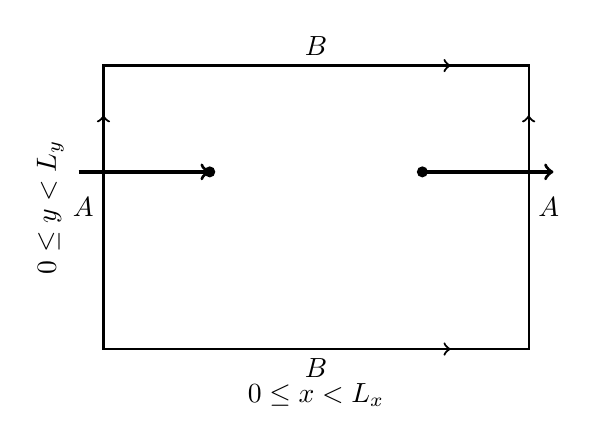
\begin{tikzpicture}[x=0.9cm,y=0.9cm]
\draw[thick] (0,0) rectangle (6,4);
\draw[->,thick] (0,0.7) -- (0,3.3);
\draw[->,thick] (6,0.7) -- (6,3.3);
\draw[->,thick] (1.1,0) -- (4.9,0);
\draw[->,thick] (1.1,4) -- (4.9,4);
\node[left] at (0,2) {$A$};
\node[right] at (6,2) {$A$};
\node[below] at (3,0) {$B$};
\node[above] at (3,4) {$B$};
\draw[->,very thick] (4.5,2.5) -- (6.35,2.5);
\draw[->,very thick] (-0.35,2.5) -- (1.5,2.5);
\fill (4.5,2.5) circle (2pt);
\fill (1.5,2.5) circle (2pt);
\node at (3,-0.65) {$0\leq x<L_x$};
\node[rotate=90] at (-0.75,2) {$0\leq y<L_y$};
\end{tikzpicture}
\caption{فضاء دوري ثنائي الأبعاد: تُطابَق الحواف التي تحمل التسمية نفسها، بحيث إن الجسيم الذي يعبر إحدى الحواف يعاود الظهور عند النقطة المناظرة على الحافة المقابلة.}
\end{figure}

\begin{classroomqa}
\lecturetimestamp{01:50:58}
\audiencequestion{هل يمثّل البناء الدوري الفضاء، أم الأجسام فيه؟}
\lecturerresponse{إنه يمثّل الفضاء. وتعيش الأجسام والحقول في ذلك الفضاء وتخضع لعلاقات التطابق فيه. وتُفرض الدورية للتحكم في مشكلة الحجم اللانهائي؛ ثم تُزال بأخذ الحجم كبيرًا واستبدال مجاميع الزخم بتكاملات.}
\end{classroomqa}

النظير الثلاثي الأبعاد هو مكعب تُطابَق فيه ثلاثة أزواج من الأوجه المتقابلة. فالوجهان الأيسر والأيمن هما نفسهما، والوجهان العلوي والسفلي هما نفسهما، والوجهان الأمامي والخلفي هما نفسهما. والجسيم الذي يعبر أيَّ وجه يعاود الظهور عبر الوجه المطابق له.\footnote{يرد المكعب الدوري وأزواجه الثلاثة من الأوجه المطابقة في 01:51:27--01:52:17. والمعادلة المعروضة لـ\(k_i\) هي إعادة كتابة على مستوى المركبات للشرط السابق \(kL=2\pi n\)، بعد تطبيقه على الاتجاهات الدورية الثلاثة.} وتخضع مركبات الزخم الثلاث لـ
\begin{equation}
k_i=\frac{2\pi n_i}{L_i},
\qquad i=x,y,z,
\end{equation}
بحيث يوجد لكل اتجاه عدد صحيح واحد \(n_i\). ويمكن تعريف فضاءات من نوع التورُس في أي عدد من الأبعاد وفق القاعدة نفسها.

\begin{figure}[t]
\centering
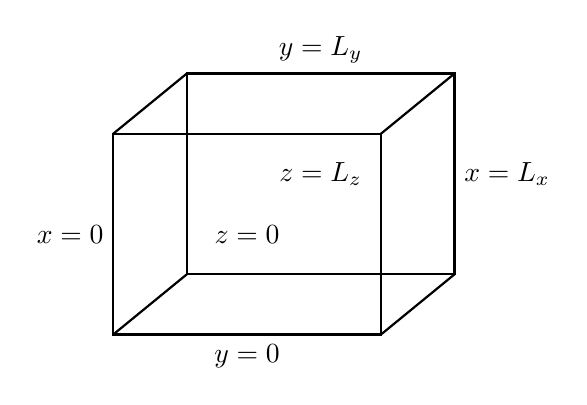
\begin{tikzpicture}[scale=0.85]
\draw[thick] (0,0) rectangle (4,3);
\draw[thick] (1.1,0.9) rectangle (5.1,3.9);
\draw[thick] (0,0) -- (1.1,0.9);
\draw[thick] (4,0) -- (5.1,0.9);
\draw[thick] (4,3) -- (5.1,3.9);
\draw[thick] (0,3) -- (1.1,3.9);
\node[left] at (0,1.5) {$x=0$};
\node[right] at (5.1,2.4) {$x=L_x$};
\node[below] at (2,0) {$y=0$};
\node[above] at (3.1,3.9) {$y=L_y$};
\node at (2,1.5) {$z=0$};
\node at (3.1,2.4) {$z=L_z$};
\end{tikzpicture}
\caption{فضاء دوري ثلاثي الأبعاد على هيئة مكعب تُطابَق فيه كلُّ زوج من الأوجه المتقابلة.}
\end{figure}

\begin{classroomqa}
\lecturetimestamp{01:52:20}
\audiencequestion{هل تختار نظرية الحقل مقياسًا شبكيًا فيزيائيًا للفضاء؟}
\lecturerresponse{هذا سؤال تخميني. ولأغراضنا العملية هنا، الفضاء متصل. والكمّات هي جسيمات، لا خلايا في شبكة مكانية. وفي بناء الدائرة، الزخم هو الذي يصبح متقطعًا؛ أما الموضع فيبقى متصلًا ودوريًا.}
\end{classroomqa}

\editorialnote{يذكر مقطع طويل متضرر أثناء الحوار حول المقياس الشبكي مقاييس بلانكية، لكنه لا يحفظ ادعاءً يمكن استخلاصه بشأن تقطّع أساسي للفضاء. ولا يُستنتج هنا مثل هذا الادعاء.}

إن تقطّع \(k\) جاء بالكامل من فرض دالة موجية دورية. وليس في ذلك دليل على أن الإحداثي \(x\) نفسه يقع على شبكة. والتساؤل عما إذا كان للفضاء بنية مجهرية أساسية أمر مشروع، لكنه مسألة منفصلة ذات طابع تخميني.

\section{الفرميونات والحقول الخارجية}

تسمح الأنماط البوزونية بأي عدد إشغال غير سالب. وتتطلب الفرميونات السلوك المعاكس: إذ يحظر مبدأ استبعاد باولي على فرميونين متماثلين أن يشغلا الحالة نفسها.

\begin{classroomqa}
\lecturetimestamp{01:55:13}
\audiencequestion{هل يؤدي استبدال المبدّلات بالمبدّلات المضادّة إلى أبسط نظرية للفرميونات؟}
\lecturerresponse{نعم، من حيث الجوهر. فالمبدّل هو \([A,B]=AB-BA\)، في حين أن المبدّل المضاد هو \(\{A,B\}=AB+BA\). والجبر الفرميوني الموافق لمؤثرات الخلق والإفناء يحقق استبعاد باولي: فلا يمكن وضع فرميون متماثل ثانٍ في حالة مشغولة بالفعل. ويؤجَّل العرض التفصيلي للنظرية.}
\end{classroomqa}

يختلف هذان الضربان بإشارة:
\begin{equation}
[A,B]=AB-BA,
\qquad
\{A,B\}=AB+BA.
\end{equation}
المبدّل مضادّ للتناظر تحت التبديل، بينما المبدّل المضاد متناظر. وإذا انعدم المبدّل المضاد، فإن
\begin{equation}
\{A,B\}=0
\quad\Longrightarrow\quad
AB=-BA.
\end{equation}
وبالنسبة إلى مثل هذا الزوج، فإن تبديل المؤثرين الفرميونيين يغيّر الإشارة. وهذا أغرب من التبادلية العادية، حيث إن \([A,B]=0\) يعطي \(AB=BA\). إن استبدال مبدّلات البوزونات بالجبر المقابل المضادّ للتبادل هو التغيير الرياضي الذي يقود إلى الفرميونات؛ ويؤجَّل بسطه التفصيلي.

المبدّلات المضادّة تعكس السلوك الإحصائي المشاهد للبوزونات. فلا يوجد تكدّس مستحثّ لفرميونات متماثلة في نمط واحد؛ فإشغال ذلك النمط يمنع فرميونًا متماثلًا آخر من دخوله. وبما أن الحالة الفرميونية الواحدة لا يمكن أن تحتوي إلا على فرميون متماثل واحد على الأكثر، فلا يُستحصل على حد حقل كلاسيكي بوضع عدد كبير اعتباطيًا منها في تلك الحالة الواحدة.

\begin{classroomqa}
\lecturetimestamp{01:58:03}
\audiencequestion{كيف يمكن أن يكون جسيم ألفا بوزونًا إذا كان مكوَّنًا من فرميونات؟}
\lecturerresponse{يمكن لمركّب مرتبط يحتوي عددًا زوجيًا من المكوّنات الفرميونية أن يتبع إحصاءات بوزونية. ووضع عدة بوزونات مركّبة من هذا النوع في الحالة الكلية نفسها ليس هو نفسه وضع مكوّناتها الفرميونية المفردة في حالة واحدة متماثلة لجسيم مفرد.}
\end{classroomqa}

تتعلق إحصاءات المركّب بالجسم المرتبط ككل. ولذلك يمكن للمكوّنات الفرميونية أن تتحد في جسم يتصرف كبوزون من دون انتهاك مبدأ الاستبعاد بالنسبة إلى المكوّنات.

\begin{classroomqa}
\lecturetimestamp{01:58:33}
\audiencequestion{كيف تُضمَّن الحقول الخارجية؟}
\lecturerresponse{لم يُضمَّن حتى الآن أي حقل خلفية خارجي في هذا البناء. ويمكن تعيين مثل هذا الحقل بوصفه حقلًا كلاسيكيًا، أو تمثيله كمّيًا بحالة تحتوي على عدد كبير من الكمّات.}
\end{classroomqa}

لكي يتفق الوصفان، يجب أن تكون الحالة ذات الإشغال الكبير مُحضَّرة على نحو مناسب ومتسقة الطور؛ وعدد الجسيمات وحده غير كافٍ.\footnote{يوفر هذا الحوار مقياس الكثرة في عدد الكمّات. ويُذكر هنا اتساق الطور بوصفه الشرط الإضافي الذي يمنع أن يُظن أن الإشغال الكبير وحده حقل كلاسيكي.} في ذلك النظام شبه الكلاسيكي تتفق آثارهما حتى انحرافات كمومية صغيرة. وهذا شرط اتساق أساسي. يجب أن يصف الحقل الكهرومغناطيسي فوتونات منفصلة عندما تكون الكمّات المفردة مهمة، ومع ذلك فلا بد أن تعيد حالة تحتوي على كثير من الفوتونات ومتسقة الطور على نحو مناسب إنتاج التأثير المألوف لموجة كهرومغناطيسية كلاسيكية.